\documentclass[a4paper, 11pt]{article}
\usepackage{geometry}
\usepackage{indentfirst}
\usepackage{setspace}
\usepackage{amsmath}
\usepackage{graphicx}
\usepackage{wrapfig}
\usepackage{caption}
\usepackage{indentfirst}
\usepackage{amssymb}
\usepackage{float}


\graphicspath{ {./images/} }
\geometry{left=2.5cm, right=2.5cm, top=2.5cm, bottom=3cm}

\begin{document}
	% Upload all the source files and a report containing:
	% Answer to theoretical questions,
	% a brief description of the methods,
	% some comments to the results
	% all the outputs.
	
	\title{Exercise \# 1. Numerical methods for ODES. }
	\author{{\small Alexandre Rodrigues (2039952)}}
	\date{\today}
	
	\maketitle
	
	\section*{Intro}
	%
	
	\section*{Methods}
	% Brief description of the methods
	
	
	\section*{Answers}
	% answer to theoretical questions
	\subsection*{Question 1}
	%....
	\begin{figure}[H]
		\centering
		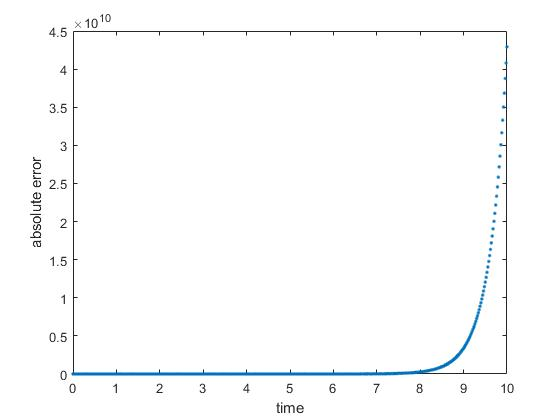
\includegraphics[width=\linewidth]{ex1_fe.jpg}
		\caption{Absolute error in function of time using Forward Euler method to compute y(1)}
		\label{fig:ex1_fe}
	\end{figure}
	
	We got a maximum error of $4.2916 \times 10^{10}$...
	
	\begin{figure}[H]
		\centering
		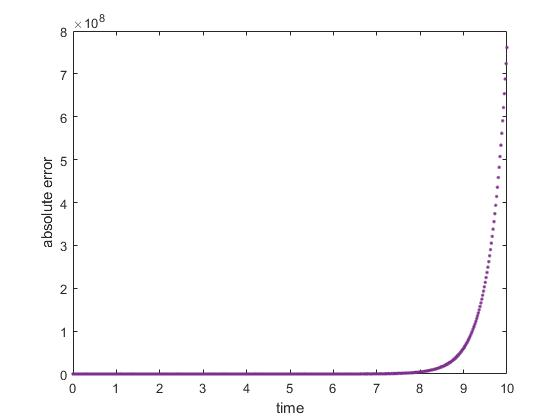
\includegraphics[width=\linewidth]{ex1_rk4.jpg}
		\caption{Absolute error in function of time using RK4 method to compute y(1)}
		\label{fig:ex1_rk4}
	\end{figure}
	
	We got a maximum error of $4.3146 \times 10^{10}$...
	
	%d)
	\subsubsection*{Comment the different behavior observed by the numerical method.}
		
	
	\subsection*{Question 2}
	\begin{figure}[H]
		\centering
		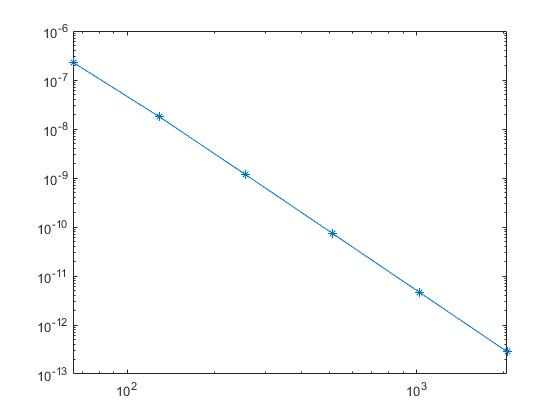
\includegraphics[width=\linewidth]{ex2.jpg}
		\caption{LogLog plot of the error as a function of the number of steps.}
		\label{fig:ex2}
	\end{figure}
	
	\begin{table}[H]
		\centering
		\begin{tabular}{c|c}
			\textbf{$h$}& \textbf{error}   \\ \hline
			$ 3.125000\times 10^{-2} $ & 25.7142859434702 \\ \hline
			$ 1.562500\times 10^{-2} $ & 25.7142857321434 \\ \hline
			$ 7.812500\times 10^{-3} $ & 25.7142857154459 \\ \hline
			$ 3.906250\times 10^{-3} $ & 25.7142857143588 \\ \hline
			$ 1.953125\times 10^{-3} $ & 25.7142857142903 \\ \hline
			$ 9.765625\times 10^{-4} $ & 25.7142857142860 \\ \hline
		\end{tabular}
	\end{table}
	
	The error reduces with the increase in the number of steps due to the decrease of $h$ as expected in theory. $\ldots$		
	
	\subsection*{Question 3}
	% Nothing done....
	
	\subsection*{Question 4}
	%....
	%a) stabilty? how?
	%b) Nothing done....
	%c) Nothing done....
	
	\subsection*{Question 5}
	\begin{figure}[H]
		\centering
		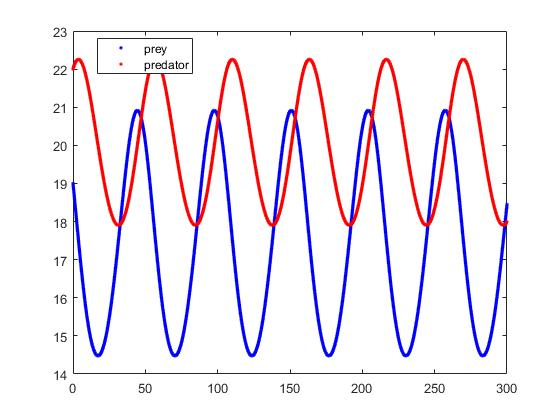
\includegraphics[width=\linewidth]{ex5.jpg}
		\caption{Evolution of the number of preys and predators.}
		\label{fig:ex5}
	\end{figure}
	
	
	
	
	
	\section*{Results}
	% comments to the results
	
	
	\section*{Outputs}
	
	
	
\end{document}



